\documentclass[12pt]{ut-thesis}

\degree{Doctor of Philosophy}
\department{Molecular Genetics}
\gradyear{2017}
\author{Jochen Weile}
\title{An atlas of variant effects in human disease genes}

\newcommand{\gene}[1]{\textit{#1}}

%% List only down to subsections in the table of contents;
%% 0=chapter, 1=section, 2=subsection, 3=subsubsection, etc.
\setcounter{tocdepth}{2}

%% Make each page fill up the entire page.
\flushbottom


%%%%%%%%%%%%      MAIN  DOCUMENT      %%%%%%%%%%%%

\begin{document}


\begin{preliminary}

\maketitle

%% There should be NOTHING between the title page and abstract.
%% However, if your document is two-sided and you want the abstract
%% _not_ to appear on the back of the title page, then uncomment the
%% following line.
%\cleardoublepage

\begin{abstract}
%% (At most 350 words for Ph.D.)

\end{abstract}

%\begin{dedication}

%\end{dedication}

\begin{acknowledgements}
The author gratefully acknowledges funding by the National Institutes of Health, the Canadian Excellence Research Chair, the Canadian Center for Advanced Research and the Ontario Ministry of Research and Innovation. The author would also like to thank Fritz Roth, Atina Cote, Jennifer Knapp, Song Sun, Marta Verby, Yingzhou Wu, Cassandra Wong, Fan Yang, Carles Pons, Natascha van Lieshout, Anjali Gopal,  Guihong Tan, Joseph Mellor, Brenda Andrews, Charles Boone, Nidhi Sahni, Marc Vidal, and David Hill for their collaboration.
\end{acknowledgements}

\tableofcontents

%\listoftables

%\listoffigures

%% You can add commands here to generate any other material that belongs
%% in the head matter (for example, List of Plates, Index of Symbols, or
%% List of Appendices).

%% End of the preliminary sections: reset page style and numbering.
\end{preliminary}


%% Introduction: Length: 25-30 pages.
%%  * Relevant background, 
%%  * Outline of state of knowledge, 
%%  * emphasize outstanding questions 

\chapter{Introduction}

Given the constantly improving cost and speed of genome sequencing, it is reasonable to expect that within the coming decades personal genomes will be known for a substantial part of the global populace. Unfortunately, our limited ability to interpret the variation found within them stands in stark contrast with this development. Even when limiting ourselves to mutations in coding regions of the genome, the effects of most missense variants are not known. While a number of computational approaches exist to make predictions as the effects of coding variants, they are currently not reliable enough for clinical use. Laboratory assays by comparison produce more trustworthy results, but until recently did not scale to the space of all possible mutations. The development of Deep mutational scanning~\cite{fowler_high-resolution_2010} has now made this endeavour possible. In the following sections, each of these issues will be discussed in detail.

\section{The Genotype-Phenotype Problem}

Linking genotype to phenotype is a very difficult problem. The part of the human genome we understand best are protein-coding genes, yet they only constitute a minuscule fraction the whole. Impacts of mutations in other functional elements such as introns, untranslated regions of genes, or regulatory sequences, are more difficult to assay, not to mention the vast stretches of intragenic space. While one might expect the latter to not bear functional significance a priori, its importance is nonetheless highlighted by the the fact that a large number of loci identified as correlated with diseases in genome-wide association studies (GWAS) are found within these regions\todo{Find citation}.
But even for protein-coding sequences the problem is far from simple. Alleles that behave according to the Mendelian model are the exception. Most phenotypes are complex, i.e. emerge through the interplay of many different genetic or environmental factors. Conversely, many genes are also pleiotropic, i.e. they are involved more than one mechanism. Thus, a mutation found in one person may not have the same effect as in another---a phenomenon called incomplete penetrance. Similarly, two different mutations within the same coding sequence need not have the same effect either. Depending on how the translated protein is affected (catastrophic folding failure, alteration of a molecular interaction interface or active site, or a subtle change on an unused surface) the effects may differ in severity or in rare cases even in the emergence of new behaviours.

%Clinical perspective on the genotype-phenotype problem
Given the much greater difficulty of interpreting non-coding regions, clinical applications have so far largely concentrated on protein-coding genes. Sequencing panels for known disease-associated genes and even whole-exome sequencing (WES) are widely commercially available. A number of different standards for classifying mutations with respect to their potential health impacts have been proposed. Most prominently, the American College of Medical Genetics and Genomics (ACMG) standard~\todo{find citation}. It defines categories stretching from ``pathogenic'' via ``variant of uncertain significance'' (VUS) to ``benign''. Even though the mutational landscape for a handful of genes, such as \gene{BRCA1} are explored better than others due to their high monetization potential~\cite{cheon_variants_2014}, the vast majority of clinical variants are currently classified as VUS. For example, over 98\% of missense variants for a gene panel assessing germline cancer risk variants~\cite{maxwell_evaluation_2016} have been discarded as VUS. Not only can these uncertainties unduly burden patients with unnecessary anxiety, they also call into question the value of sequencing in the clinic if the majority of findings are not actionable. With increasing use of WES, this problem is only going to get worse. According to  the 1000 Genomes Project data, every person carries 100-400 missense variants that are so rare that they have likely never been seen before in the clinic~\cite{the_1000_genomes_project_consortium_global_2015}. In the absence of previous observations they would automatically be added to long list of VUS.

\section{\textit{In silico} approaches to variant function assessment}
\label{insilicoIntro}

A number of algorithms exist that offer predictions as to the deleteriousness of mutations, the most prominent ones being PolyPhen-2~\cite{adzhubei_predicting_2001}, SIFT~\cite{ng_predicting_2001} and PROVEAN~\cite{choi_predicting_2012}. PolyPhen-2 uses a machine learning method using evolutionary conservation and protein structural features. It uses a set of previously reported pathogenic alleles as a positive training set and differences between human genes and their mammalian homologues as a negative training set. SIFT (Sorting Intolerant From Tolerant) by contrast only uses evolutionary conservation. The tool uses multiple sequence alignments to calculate position-specific score matrices for each gene which are then normalized and transformed into probability values. PROVEAN (PROtein Variation Effect ANalyzer) similarly only takes into account sequence alignments. However, rather than just computing a position-specific score, PROVEAN calculates the difference in alignment quality between using the wildtype or variant sequence against clusters of homologous sequences. The average distance is then interpreted as indicative of the deleteriousness of the variant. 

While the three tools succeed in making good predictions, their reliability is unfortunately still not high enough to serve as a basis of clinical decision making. Song Sun and other members of the Roth Lab recently performed an independent comparison of these tools on a set of well established disease-causing variants as well as rare polymorphisms with no known disease association~\cite{sun_extended_2016}. A high precision (the fraction of correct classifications out of all positive classifications) can be considered especially important when considering taking clinical action based on a prediction. When compared at a minimum precision level of 90\%, PolyPhen-2 and PROVEAN only reach a sensitivity of 19\% and 21\%, respectively (where sensitivity is defined as the fraction of correct classifications out of all real existing disease variants). SIFT was not even capable of achieving 90\% precision at any score threshold.

\section{Laboratory approaches to variant function assessment}

An alternative to computational prediction for variant assessment is the use of laboratory assays. Many different types of assays exist that can yield potential insight into the effects of missense variants on protein function. However many of them, such as enzymatic activity assays need to be performed one by one and are not easily scalable. Two particularly useful assays in this respect are Yeast-2-Hybrid and functional complementation.

Yeast-2-Hybrid (Y2H)~\cite{fields_novel_1989} is a binary protein interaction assay performed within the yeast \species{Saccharomyces cerevisiae}. It is based on the reconstitution of two fragments of the transcription factor Gal4. The Gal4 protein comprises two domains: A DNA-binding (DB) domain and an activating domain (AD) both are required for it to successfully associate with its cognate promoter region and induce expression of a reporter gene downstream of the promoter. When two proteins X and Y are fused to the DB and AD domain respectively, an prospective interaction between X and Y leads to the reconstitution of the transcription factor and subsequently to reporter expression. In most cases, the reporter is an auxotrophy marker, such as \gene{HIS3}, thus linking the ability of the two proteins to interact with each other to the ability of the yeast strain to grow on selective media. When comparing different variants of the same protein interacting with the same partner, reporter expression has even been shown to be proportional to binding affinity~\cite{yang_protein-peptide_1995}. This allows for quantitative interpretation of Y2H results under these specific circumstances. 

Y2H does however suffer from a number of drawbacks. Due to the the transcription factor needing to physically associate with DNA, any protein to be examined needs to be able to enter the nucleus. While the DB domain already contains a nuclear localization sequence (NLS), the AD ORF is often the fused with an additional NLS. However, this does not work for every protein~\cite{van_criekinge_yeast_1999}. A particular problem are membrane proteins which generally cannot enter the nucleus at all. A variant of Y2H, MYTH exists for these proteins~\cite{snider_split-ubiquitin_2010}. It has been estimated that Y2H has an overall assay sensitivity of 20\%. That is, only one in five real existing protein interactions can be detected by Y2H~\cite{venkatesan_empirical_2009}. These levels are comparable most other binary interaction assays, such as PCA~\cite{tarassov_vivo_2008} or MAPPIT~\cite{eyckerman_design_2001}.

%Explain difference between binary and complex interactions
%Explain previous confusions about reproducibility originating from Ito et al.

When considering Y2H as an assay for variant function assessment it is important to consider that it does not measure all aspects of a protein's functionality, but rather only its ability to physically associate with a given interaction partner. Thus only variants that result either in major failures in protein folding or in changes to the binding binding interface could be detected. However, in a recent examination of the Y2H performance of common disease associated variants, we found that approximately two out of three disease variants manifest in such a way~\cite{sahni_widespread_2015}. 


\begin{figure}[h!]
	\centering
	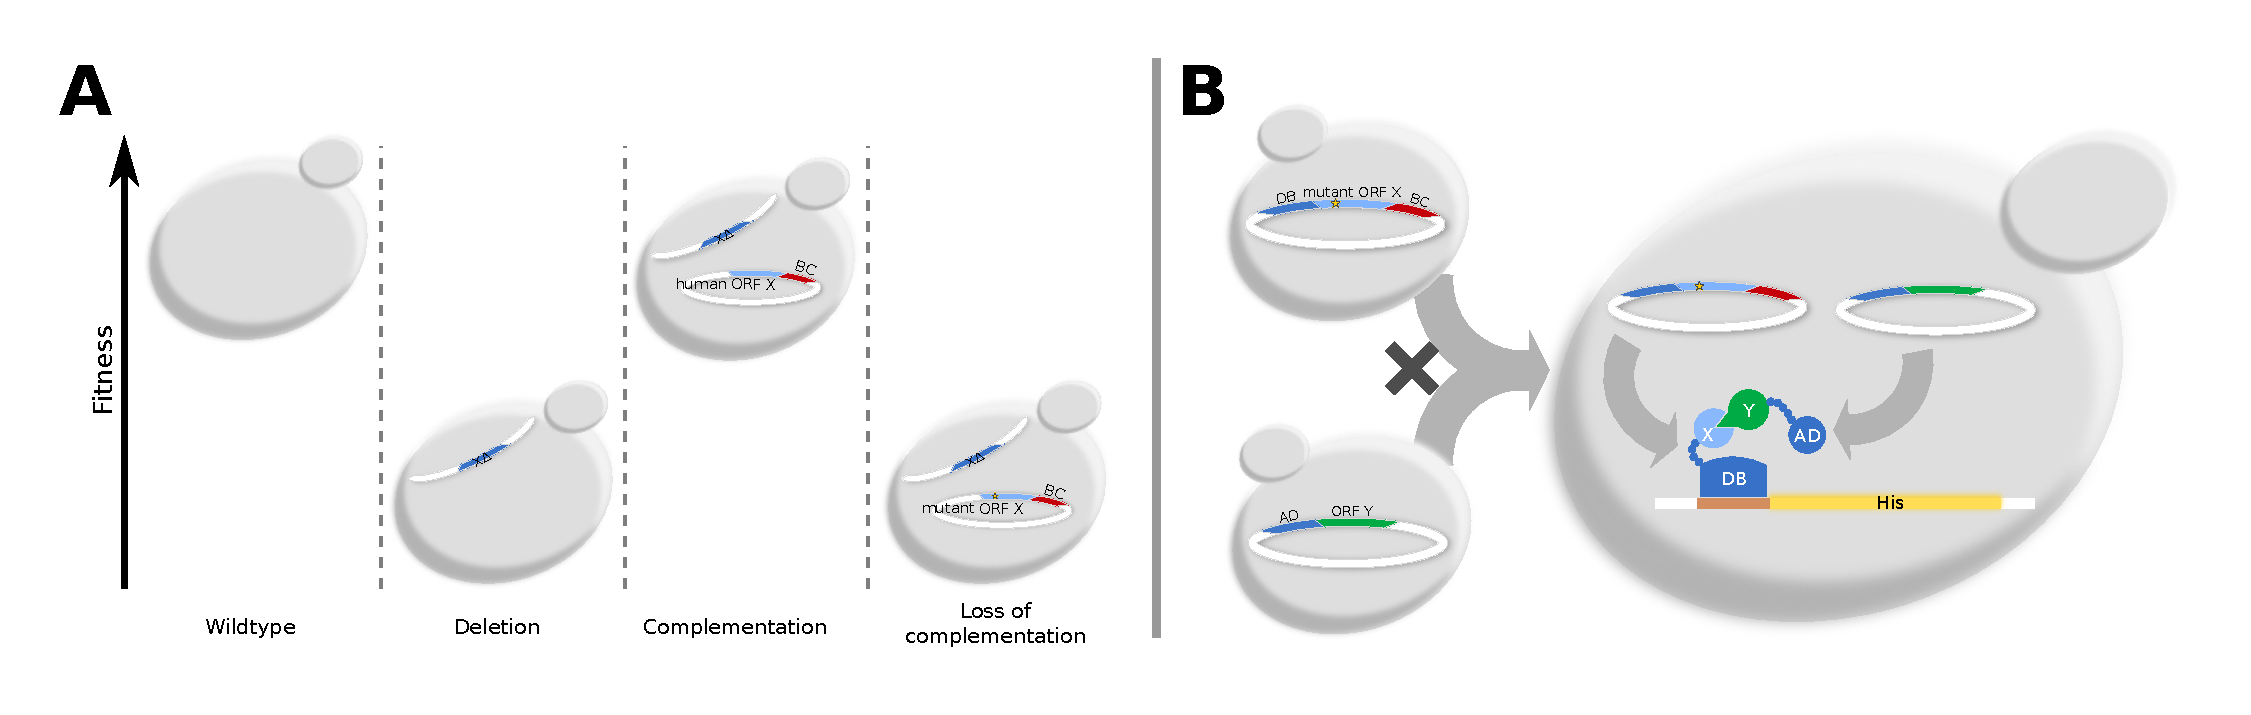
\includegraphics[width=\textwidth]{img/compl_y2h.pdf}
	\caption{Complementation and Yeast-2-Hybrid}
	\label{fig:compl_y2h}
\end{figure}
%Discuss Edgotyping?

Nonetheless, an assay that can measure the overall functionality of a protein within the cell would be preferable. Functional complementation~\cite{lee_complementation_1987} in yeast offers such an option. It based on the premise that some human genes can be used to rescue the deletion of their orthologues in yeast. That is, a fitness defect resulting from the inactivation of the yeast gene is alleviated by the artificial expression of the human gene. Therefore, any relative changes in fitness upon expressing a variant of the human gene can be interpreted as the variant's effect on the protein's overall ability to function. Song Sun and other members of the Roth Lab have recently examined the applicability of functional complementation in yeast to the assessment of disease variants~\cite{sun_extended_2016}. They have found an astonishing predictive capacity despite yeast and humans being diverged by a 1.5 billion year. Yeast complementation outperformed \textit{in silico} methods like PolyPhen-2 and PROVEAN in terms of disease variant prediction by a wide margin. At the 90\% specificity threshold discussed in section~\ref{insilicoIntro}, the complementation assay achieved a sensitivity of over 60\% (as compared to 19\% and 21\% for the two \textit{in silico} methods, respectively).

The only major drawback of yeast complementation is that currently only 60 human genes have been found to be amenable to the assay~\cite{sun_extended_2016}. %mention future outlook on human cell complementation and CRISPR? 

%Mention Phage display?


\section{Deep Mutational Scanning}

Complementation and Y2H promise to be useful tools in the classification of variants of uncertain significance. Yet applying them to retroactively test variants only once they have been found in the clinic would be a slow process. Instead, a proactive approach could prove to be more useful: Building an atlas of the functional effects of all possible variants before they are even seen in the clinic. This would require a massive parallelization of the assays. Indeed such parallelization efforts have previously been described, albeit not for the classification of VUS. Fowler and Fields have pioneered a technology called Deep Mutational Scanning (DMS)~\cite{fowler_high-resolution_2010}, which can be thought of as a natural extension to Alanine Scanning~\cite{cunningham_high-resolution_1989}, expanding it into the space of all possible amino acid changes. Fowler and Field's original paper has since inspired a fair number of similar efforts by other groups~\cite{ernst_coevolution_2010,fujino_robust_2012,adkar_protein_2012,mclaughlin_jr_spatial_2012,schlinkmann_critical_2012,whitehead_optimization_2012,traxlmayr_construction_2012,wu_systematic_2013,roscoe_analyses_2013,starita_activity-enhancing_2013,procko_computational_2013,tinberg_computational_2013,jiang_latent_2013,kim_high-throughput_2013,melamed_deep_2013,forsyth_deep_2013,wagenaar_resistance_2014,firnberg_comprehensive_2014,olson_comprehensive_2014,melnikov_comprehensive_2014,thyagarajan_inherent_2014,stiffler_evolvability_2015,doud_site-specific_2015,kitzman_massively_2015,starita_massively_2015,mishra_systematic_2016,doud_accurate_2016,mavor_determination_2016} (See Table~\ref{table:DMSstudies}). However, when considering these studies in the context of VUS classification, a number issues become apparent. Many of these have primarily used DMS in the context of biochemistry. The assays underlying different DMS studies are quite diverse and measure different aspects of a protein’s behaviour. As a consequence, they cannot be easily compared with each other. In addition, the achieved coverage of possible amino acid changes varies from map to map. Finally, many maps to do not control the quality of measurements. Therefore, the confidence levels underlying different parts of these maps are often unknown. A generalized framework that would allow for the construction of comparable, high-quality maps representing overall protein function would be of great utility.


\begin{landscape}
\begin{table}
	\centering
	\caption{Previous DMS studies}
	\label{table:DMSstudies}
	\begin{tabular}{l l l l l l l}
\textbf{Year} & \textbf{Authors} & \textbf{Protein} & \textbf{Region} & \textbf{Saturation} & \textbf{Selection} \\ \hline \hline
2010 & Fowler~\etal~\cite{fowler_high-resolution_2010} & YAP65 & WW domain & Very high & Phage display \\  
2010 & Ernst~\etal~\cite{ernst_coevolution_2010} & Synthetic protein & PDZ domain & ? & Phage display \\ 
2012 & Fujino~\etal~\cite{fujino_robust_2012} & Fab antibody fragment & fragment & Very high & Ribodisplay \\ 
2012 & Adkar~\etal~\cite{adkar_protein_2012} & Ccdb & whole protein & ? & Toxin activity in \species{E.~coli}\\ 
2012 & McLaughlin~\etal~\cite{mclaughlin_jr_spatial_2012} & PSD95 & PDZ domain & Very high & B2H+FACS (\species{E.~coli})\\ 
2012 & Schlinkmann~\etal~\cite{schlinkmann_critical_2012} & GPCR & whole protein & High & FACS (\species{E.~coli})\\ 
2012 & Whitehead~\etal~\cite{whitehead_optimization_2012} & Synthetic protein & whole protein & Very high & Yeast display \\ 
2012 & Traxlmayr~\etal~\cite{traxlmayr_construction_2012} & IgG1 & CH2/CH3 domains & ? & Yeast display \\ 
2013 & Wu~\etal~\cite{wu_systematic_2013} & Neuraminidase & SNP accessible & ? & Drug resistance (H1N1)\\ 
2013 & Roscoe~\etal~\cite{roscoe_analyses_2013} & Ubiquitin & whole protein & High & Yeast growth\\ 
2013 & Starita~\etal~\cite{starita_activity-enhancing_2013} & Ub.E3 E4B & whole protein & Low & Phage display\\ 
2013 & Procko~\etal~\cite{procko_computational_2013}  & Synthetic protein & 60AA & Very high & Yeast display\\ 
2013 & Tinberg~\etal~\cite{tinberg_computational_2013}  & Synthetic protein & 40AA & High & Yeast display\\ 
2013 & Jiang~\etal~\cite{jiang_latent_2013}  & Hsp90 & substrate binding loop & Very high & Yeast complementation\\ 
2013 & Kim~\etal~\cite{kim_high-throughput_2013}  & Mat alpha  & degron region & ? & Yeast growth\\ 
2013 & Melamed~\etal~\cite{melamed_deep_2013}  & Pab1 & RRM domain & High & Yeast complementation\\ 
2013 & Forsyth~\etal~\cite{forsyth_deep_2013}  & Antibody for EGFR & whole protein & Very high & Human cell display\\ 
2013 & Wagenaar~\etal~\cite{wagenaar_resistance_2014}  & BRAF & 77 Aas & ? & Drug resistance (Human)\\ 
2014 & Firnberg~\etal~\cite{firnberg_comprehensive_2014}  & TEM1-beta lactamase & Whole protein & High & Drug resistance (\species{E.~coli})\\ 
2014 & Olson~\etal~\cite{olson_comprehensive_2014}  & G protein (GB1) & IgG-binding domain & High & RNA display\\ 
2014 & Melnikov~\etal~\cite{melnikov_comprehensive_2014}  & APH(3′)II (kinase) & whole protein & Very high & Drug resistance (\species{E.~coli})\\ 
2014 & Thyagarajan~\etal~\cite{thyagarajan_inherent_2014}  & hemagglutinin & whole protein & ? & Viral replication (H1N1)\\ 
2015 & Stiffler~\etal~\cite{stiffler_evolvability_2015}  & TEM1 Beta-lactamase & whole protein & Very high & \species{E.~coli} growth\\ 
2015 & Doud~\etal~\cite{doud_site-specific_2015}  & influenza nucleoprotein & whole protein & ? & Viral replication (H1N1)\\ 
2015 & Kitzman~\etal~\cite{kitzman_massively_2015}  & Gal4 & DB domain & Very high & Yeast growth \\ 
2015 & Starita~\etal~\cite{starita_massively_2015}  & BRCA1 & RING domain & Low & Y2H + E3 activity\\ 
2016 & Mishra~\etal~\cite{mishra_systematic_2016}  & Hsp90 & ATPase domain & Very high & Yeast growth\\ 
2016 & Doud~\etal~\cite{doud_accurate_2016}  & Hemagglutinin & whole protein & ? & Viral replication (H1N1)\\ 
2016 & Mavor~\etal~\cite{mavor_determination_2016}  & Ubiquitin & whole protein & Very high & Yeast growth
\end{tabular}
\end{table}
\end{landscape}


Nonetheless, the existing studies allow for a survey of available methodologies and the structures they have in common. Deep Mutational Scanning can be broken down into a number of experimental and computational steps: (1) Mutagenesis; (2) Library construction; (3) Selection of functional mutants; (4) Sequencing of the pre- and post-selection libraries; and (5) Statistical analysis to determine the quantitative enrichment resulting from the selection. 

\begin{table}
	\centering
	\caption{Experimental steps in Deep Mutational Scanning}
	\label{table:DMSphases}
	\begin{tabular}{l p{10cm}}
	\textbf{Step}                & \textbf{Options} \\ \hline \hline
	Step 1: Mutagenesis          & Error-prone PCR, Kunkel, Oligo Array, Gene Synthesis\\ 
	Step 2: Library construction & Gibson Assembly, Gateway\\ 
	Step 3: Selection            & Complementation, Y2H, Phage display, Viral replication\\ 
	Step 4: Sequencing           & BarSEQ, Deep Sequencing\\ 
	Step 5: Analysis             & Enrich2\\ 
	\end{tabular}
\end{table}

The first step---mutagenesis---has been performed in different ways by different groups. The simplest method is error-prone PCR amplification~\cite{firstErrorPronePCR,mohan_pcr_2011}. While this has the advantage of being an inexpensive and facile procedure, it will only result in the generation of point mutations and as such will not generate all possible amino acid replacements. One may argue that the evaluation of VUS does not require insight into mutations outside of this set, however at the expense of potentially valuable biochemical insights. Another method often employed is Kunkel mutagenesis~\cite{kunkel_rapid_1985}. Originally developed as a method for simple site-directed mutagenesis, it can be scaled up to address a combination of multiple sites at once. It uses a special strain of \species{E.~coli} that has been modified to produce high levels of uradine and lacks the ability to excise uracil bases from DNA. A phage vector carrying the desired template sequence is transfected into the cells resulting in its replication with a high uracil incorporation rate. The thus uracilated template can be PCR amplified with primers containing the mutations of interest and subsequently amplified in regular \species{E.~coli} which will degrade the uracilated template, thus enriching the mutant copies. %More
A more recent development is the use of custom oligonucleotide arrays covering all possible (or desired) options of codon changes~\cite{kitzman_massively_2015}. These can then be used in linear amplification reactions with the gene template. While this option allows for the precise control of desired mutations, it is currently too expensive to be applicable at genome-scale. Similarly, mutagenesis libraries are becoming commercially available via gene synthesis~\cite{kosuri_scalable_2010}. While this method is certainly the most convenient, it is by far the most expensive option. A middle ground can be found in methods that employ amplification with oligonucleotides carrying degeneracy codons~\cite{pal_methods_2005}. Particularly popular is the use of NNK and NNS degeneracies, which have long been used in biochemistry~\cite{scott_searching_1990,barbas_semisynthetic_1992}. Here, S denotes Guanine or Cytosine and K denotes Guanine or Thymine in the third position of the codon. While either of these codes only allow 32 of all 64 possible codons to be formed, they do cover all 20 possible amino acids, while avoiding two of the three possible stop codons (opal and ochre).

Library construction is the second step in any DMS experiment. The choice of method in this step is dependent on the type of selection and sequencing used in the later steps. Some methods require mutants to be tagged with molecular barcodes, i.e. short unique DNA sequences inserted at a known location that allow identification of a molecule with just a single sequencing read. While the use of barcodes greatly simplifies the readout of the selection result it does require that the contents of the library are catalogued at the time of construction.

Step three of a DMS procedure is the selection of mutants that pass a given assay. In most cases, assays are designed to test for protein protein interactions, for example via Y2H or phage display~\todo{REF}. In other cases it may be overall protein function, as measured by complementation or in cases of viral proteins, the ability of the virus to replicate.

The fourth step in the procedure is sequencing. 

%The original method used phage display as a method of selection on an exhaustive library of mutant proteins followed by deep sequencing to identify which mutant proteins were enriched in the process. While the original method was developed as an extension to alanine scanning~\cite{alanineScanning} in the pursuit of biochemical insights, it can certainly be adapted to work with other selection methods such as Y2H and complementation. Indeed, \todo{Who?} and colleagues have recently adapted it to the use of complementation as a means of selection.
% \section{Edgotyping}

\section{Background: The Sumoylation Pathway}
\label{intro:sumoylation}

In the following chapters, we will evaluate the performance of sequence-function technology such as Deep Mutational Scanning with respect to its ability to detect effects not only on overall function but individual subfunction. Beyond the amenability of the proteins to the employed assays, an ideal testing ground would be comprised of a biological system that is both mechanistically complex and has been well studied previously in terms of structure and mechanism. The Sumoylation life cycle does not only fulfill these criteria, but is also of great biological importance. Sumoylation is a protein modification in which a small ubiquitin-like modifier (SUMO) is covalently attached to target proteins in order to modulate their behavior, especially in terms of localization and physical interactions~\cite{sumoylation}. Sumoylation plays an important role in a large number of cellular processes. It is therefore not surprising that the core members of the pathway are essential genes~\todo{REF}.

\begin{figure}
	\centering
	\includegraphics[width=\textwidth]{img/sumoylation_steps.pdf}
	\caption{Steps in the sumoylation cascade. SENP protease matures a SUMO precursor by cleaving off its four C-terminal residues. In the activation step, the E1 complex forms a thioester bond  between SUMO and one of its cysteine residues under ATP consumption. It then transestereficates SUMO to the E2. The E2 recognizes potential targets via their $\Psi$KXE motif. With the help of an E3, SUMO is then ligated to the central lysine within that motif. SENP proteases can reverse the process by hydrolysing this new peptide bond. Images are based on the following PDB structures: \texttt{2G4D}~\cite{Xu2006}, \texttt{3KYC}~\cite{Olsen2010}, \texttt{4W5V}~\cite{ReiterEtAl}, \texttt{3UIP}~\cite{Gareau2012}}
	\label{fig:sumoylation_steps}
\end{figure}

Despite employing a distinct set of proteins compared to the ubiquitination machinery, the sumoylation pathway bears many close similarities. Analogously to ubiquitin, an enzymatic cascade of proteases, E1, E2 and E3s guide SUMO through its maturation, activation, conjugation and ligation phase~\cite{sumoylation} (Figure \ref{fig:sumoylation_steps}). After expression, SUMO is matured through cleavage of four amino acids from its C-terminus, exposing a diglycine motif. In humans, this process is performed by two proteases, SENP1 and SENP2. Next, an E1 activation complex (UBA2-SAE1) forms a thioester bond between the SUMO C-terminal diglycine and a cysteine residue within the E1 protein under the consumption of ATP. An E2 conjugase (UBE2I) binds to the complex, so that the activated SUMO can be transfered to one of its own cysteine residues via transesterification. 

The thus loaded E2 can recognize potential target proteins via an exposed motif of four amino acids. The motif is generally described as $\Psi$KxD/E, i.e. a large hydrophobic residue, followed by a lysine, a spacer residue and an acidic residue~\cite{Sampson2001}. The motif is often found in an extended loop extending from the protein or in a disordered region~\todo{REF}. The central lysine within the motif enters the E2’s active site where it comes into contact with the SUMO diglycine. There, a peptide bond is formed between the lysine $\varepsilon$-amino group and the SUMO C-terminus~\cite{BernierVillamor2002}. This process can be made more efficient in the presence E3 proteins. It is interesting to note, that while only a single SUMO E2 conjugase (UBE2I) is encoded by the human genome, there is a variety of different SUMO E3 ligases. Some work by simply stabilizing the SUMO-E2 complex, while others can outright force-feed non-canonical targets to the E2~\cite{Streich2016}. 

\begin{figure}[h!]
	\centering
	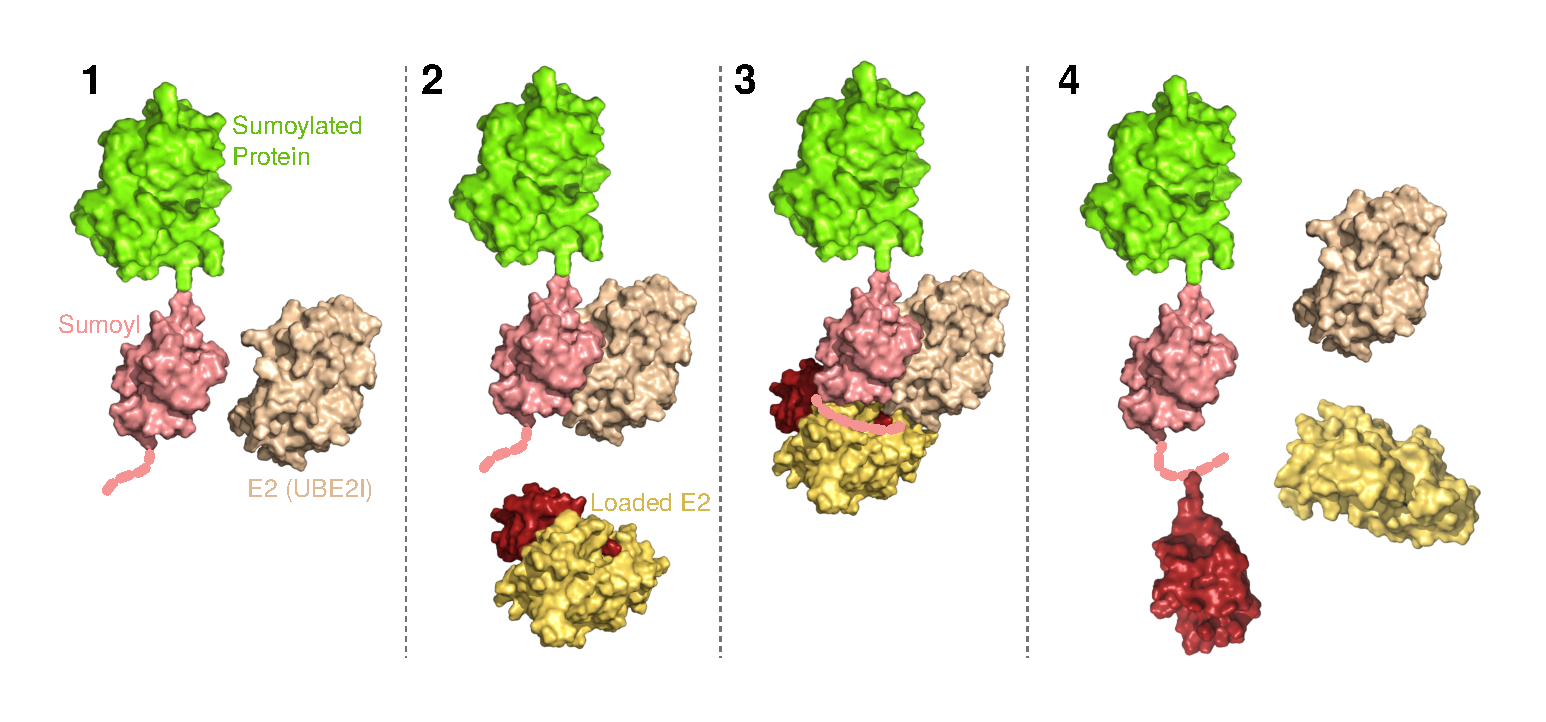
\includegraphics[width=\textwidth]{img/sumo_chaining.pdf}
	\caption{Steps in SUMO chain formation as proposed by Alontaga and colleagues~\cite{Alontaga2015}. An E2 noncovalently interacts with a SUMO modification of a target protein. A second E2 carrying a covalently bound second SUMO binds the first E2-SUMO complex, allowing for the first SUMO's N-terminal tail to enter the active site, where a lysine within the tail is forms a peptide bond with the second SUMO's C-terminus. Finally, the complex dissociates, leaving behind the newly formed SUMO chain. Images are based on the following PDB structures: \texttt{3UIP}~\cite{Gareau2012}, \texttt{4Y1L}~\cite{Alontaga2015}}
	\label{fig:sumo_chaining}
\end{figure}

Like ubiquitin, SUMO can also form chains (Figure \ref{fig:sumo_chaining}). However, of the four SUMO proteins encoded by the human genome, only SUMO2 and SUMO3 are capable of doing so, as they contain a suitable lysine residue within a disordered N-terminal tail\todo{REF}. Capili and Lima previously observed that the E2 (UBE2I) and SUMO can interact in a noncovalent manner via a distinct binding interface~\cite{CapiliLima2007}. According to a model proposed by Alontaga and colleagues~\cite{Alontaga2015} this interaction is a key mechanism in SUMO chain formation. The interaction recruits a second, SUMO-loaded E2 that interacts with the complex in such a manner that the lysine within the first SUMO's N-terminal tail can find its way into the active site of the second E2, where the second SUMO is concatenated.



Given the complexity of the Sumoylation system, especially surrounding the E2 component, an examination of sequence-structure-function relationships becomes a multifaceted problem. Mutations could in principle affect any combination of the multiple interaction interfaces which in turn contribute in complex ways to the overall cellular phenotype.
An alanine scan of the yeast SUMO E2 Ubc9 was previously performed and succeeded in identifying functionally important sites within the protein 20. Similarly, a DMS scan of ubiquitin, was previously completed 21. While both of these projects provided great insight into the biochemistry of ubiquitin-like protein pathways, neither has produced a complete map.
%Sampson2001: The small ubiquitin-like modifier-1 (SUMO-1) consensus sequence mediates Ubc9 binding and is essential for SUMO-1 modification. 
%BernierVillamor2002: Structural basis for E2-mediated SUMO conjugation revealed by a complex between ubiquitin-conjugating enzyme Ubc9 and RanGAP1.
%Streich2016: Capturing a substrate in an activated RING E3/E2–SUMO complex
%CapiliLima2007: Structure and analysis of a complex between SUMO and Ubc9 illustrates features of a conserved E2-Ubl interaction
%Alontaga2015: RWD Domain as an E2 (Ubc9)-Interaction Module
%Xu2006: http://www.biochemj.org/content/398/3/345
%Olsen et al. 2010 (Lima Lab) Active site remodelling accompanies thioster bond formation in the SUMO E1
%Katherine H. Reiter‡, Anita Ramachandran‡, Xue Xia‡, Lauren E. Boucher‡,§, Jürgen Bosch‡,§ and Michael J. Matunis‡1Characterization and Structural Insights into Selective E1-E2 Interactions in the Human and Plasmodium falciparum SUMO Conjugation Systems.


%% This adds a line for the Bibliography in the Table of Contents.
\addcontentsline{toc}{chapter}{Bibliography}
\bibliographystyle{plain}
\bibliography{thesis}

\end{document}
